%---------change this every homework
\def\yourid{yl4df}
\def\collabs{mw5ew}
\def\sources{list any sources, e.g.\ Cormen, et al, Introduction to Algorithms}
% NOTE: To specifically cite your sources, include your bibliography.bib file from
% homework 0 when LaTeXing your document (or upload it to Overleaf with this document)
% and then uncomment the penultimate last two lines of this file to display the
% bibliography.
% -----------------------------------------------------
\def\duedate{Thursday, February 27 at 11p}
\def\duelocation{via Collab}
\def\hnumber{4}
\def\course{{cs4102 - algorithms - spring 2020}}%------
%-------------------------------------
%-------------------------------------

\documentclass[10pt]{article}
\usepackage[colorlinks,urlcolor=blue]{hyperref}
\usepackage[osf]{mathpazo}
\usepackage{amsmath,amsfonts,graphicx}
\usepackage{latexsym}
\usepackage[top=1in,bottom=1.4in,left=1.25in,right=1.25in,centering,letterpaper]{geometry}
\usepackage{color}
\definecolor{mdb}{rgb}{0.1,0.6,0.4} 
\definecolor{cit}{rgb}{0.05,0.2,0.45} 
\pagestyle{myheadings}
\markboth{\yourid}{\yourid}
\usepackage{clrscode}
\usepackage{url}
\usepackage{tabularx,booktabs}
\newcolumntype{Y}{>{\centering\arraybackslash}X}

\newenvironment{proof}{\par\noindent{\it Proof.}\hspace*{1em}}{$\Box$\bigskip}
\newcommand{\handout}{
   \renewcommand{\thepage}{Homework \hnumber~-~\arabic{page}}
   \noindent
   \begin{center}
      \vbox{
    \hbox to \columnwidth {\sc{\course} \hfill}
    \vspace{-2mm}
       \hbox to \columnwidth {\sc due \MakeLowercase{\duedate} \duelocation\hfill {\Huge\color{mdb}H\hnumber(\yourid)}}
      }
   \end{center}
   \vspace*{1mm}
   \hrule
   \vspace*{1mm}
    {\footnotesize \textbf{Collaboration Policy:} You are encouraged to collaborate with up to 4 other students, but all work submitted must be your own {\em independently} written solution. List the computing ids of all of your collaborators in the \texttt{collabs} command at the top of the tex file. Do not share written notes, documents (including Google docs, Overleaf docs, discussion notes, PDFs), or code.  Do not seek published or online solutions for any assignments. If you use any published or online resources (which may not include solutions) when completing this assignment, be sure to cite them. Do not submit a solution that you are unable to explain orally to a member of the course staff. Any solutions that share similar text/code will be considered in breach of this policy. Please refer to the syllabus for a complete description of the collaboration policy.
   \vspace*{1mm}
    \hrule
    \vspace*{2mm}
    \noindent
    \textbf{Collaborators}: \collabs\\
    \textbf{Sources}: \sources}
    \vspace*{2mm}
    \hrule
    \vskip 2em
}
\newcommand{\solution}[1]{\medskip\noindent\textbf{Solution:}#1}
\newcommand{\bit}[1]{\{0,1\}^{ #1 }}
%\dontprintsemicolon
%\linesnumbered
\newtheorem{problem}{\sc\color{cit}problem}
\newtheorem{practice}{\sc\color{cit}practice}
\newtheorem{lemma}{Lemma}
\newtheorem{definition}{Definition}
\newtheorem{theorem}{Theorem}

\newcommand{\Z}{\mathbb{Z}} % This might be useful for Integers!

\begin{document}
\thispagestyle{empty}
\handout

%----Begin your modifications here

\begin{problem} Disney+ \end{problem}

Disney+ has gained in popularity since its release last Fall.  However, the executives are worried about password sharing and have asked you to look into the problem.  They come to you with a list of $n$ total login instances and provide an \emph{equivalence tester} that tells you, in constant time, if two logins were produced from the same account.  Specifically, due to privacy concerns, they do not share full login details and will only allow your algorithm to compare the login equivalence of two of the items in the list at a time.

Design an algorithm to determine if there exists a set of at least $\lceil \frac{n}{2} \rceil$ logins that were from the same account.  Your algorithm must solve this problem in $\Theta(n \log n)$ total invocations of the \emph{equivalence tester} Disney provided.

\vspace*{.1in}
First, for ease of explanation, let us define that if at least $\lceil \frac{n}{2} \rceil$ logins that were from the same account among $n$ total login instances, we call the logins as the \emph{majority login}.

We denote the list of $n$ total login instances as $l$ and split it as $l_1$ and $l_2$. We know that if $l$ has the majority login, then the majority login must appear in $l_1$ or $l_2$ or both. Based on this principle, we designed the algorithm as follows:
\\
The algorithm starts by splitting the array in half repeatedly and recursively calling itself on each half. The base case is when when have only one login, the login becomes the majority login of the 1-element array. For other cases, it will get return values from its two recursive calls on its two sub list. Then we will encounter three scenarios. 
\\First, if the majority logins from sub lists come from the same account by the test of \emph{equivalence tester}, then that login becomes the majority login of the combined list and the algorithms returns True with that login. The run-time is constant.
\\Second, if only one sub list has the majority login, then we run the \emph{equivalence tester} against every other logins in the combined list to determine if the login is the majority login for the combined list and the algorithm returns True with that login or False correspondingly. The run-time is linear.
\\Third, if both sub lists have the majority logins but they are different, we will run \emph{equivalence tester} for both candidates against every other logins in the combined list. If neither of them becomes the majority login of the combined list, the algorithm returns False. If either of them becomes the majority login of the combined list, the algorithm returns True with that login. If both of them becomes majority logins (i.e. account 1 has $\frac{n}{2}$ logins and account 2 has $\frac{n}{2}$ logins), the algorithm returns True with a list containing both majority logins as potential candidates. The run-time is linear

After recursively calling itself on each half, the algorithm returns True if a majority login exist or False if not.

As we can see above, at each level, the worst-case calls \emph{equivalence tester} $\Theta(n)$ times. The recurrence relation is 
\begin{align}
    T(n) = 2 T(\frac{n}{2}) + \Theta(n).
\end{align}
According to the Case 2 of the Master Theorem, we have $T(n) = \Theta(n \log n)$.
\vspace*{.25in} % here's how you add some vertical spacing!  Take this out if you don't want it.
% ------ new problem ---------------------------------------------------------------------------------
\begin{problem} Random Permutations \end{problem}

Consider the following pseudo-code for randomly permuting an array $A$ of size $n$:
\[ \mathtt{For} \ i = 0 \ \mathtt{to} \ n-1: \ \mathtt{Swap}(A[i], A[\mathtt{Random}(0,n-1)]) \]
 where $\mathtt{Random}(i,j)$ returns a random integer uniformly distributed in the range $i$ through $j$ (inclusive).
\begin{enumerate}
    \item Prove that for any choice of $n>2$, not all permutations are equally probable using this pseudo-code (hint: use decision trees)
    \begin{proof}
    Based on the algorithm given above, we have $n$ cards and each cards can be swapped to $n$ positions. This implies that we have $n^n$ leaves in the decision tree (graph shown below). As we know, the number of permutations of $n$ cards is $n!$. In order to show that for any choice of $n>2$ not all permutations are equally probable using this pseudo-code, we need to show $n!$ cannot divide $n^n$. We prove this statement by contradiction. Suppose $n!$ divides $n^n$. According to Euclid's Theorem, any integer can be expressed as the product of prime number, so we have $p$ divides $n-1$ where $p$ is a prime number and thus $p$ divides $n!$. Then we know $p$ cannot divide $n$ because $n$ and $n-1$ are co-prime for $n>2$. This implies $p$ cannot divide $n^n$. Since $n!$ divides $n^n$, then from $p$ divides $n!$, we have $p$ divides $n^n$, which causes contradiction. Thus, $n!$ cannot divide $n^n$. This means that for any choice of $n>2$ not all permutations are equally probable using this pseudo-code. 
    \end{proof}
    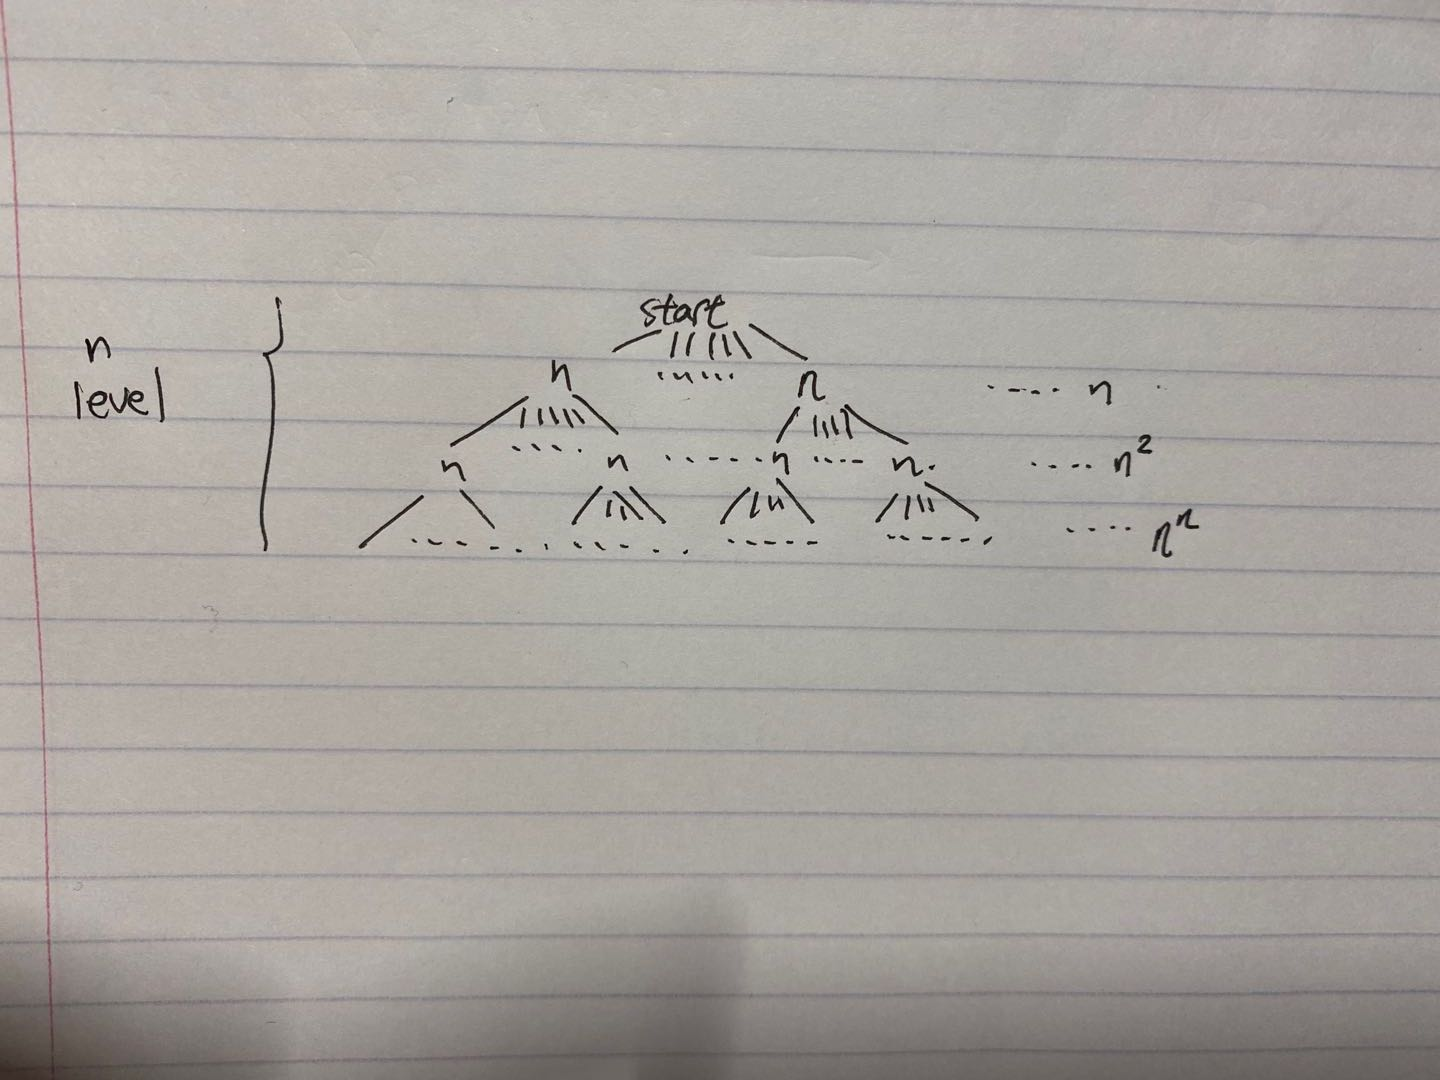
\includegraphics[scale=0.15]{pic3.jpeg}
    \item Give pseudo-code for a method to randomly permute a list without this flaw. Prove that all possible permutations are equally likely using your technique.
    
    New pseudo-code:
    \[ \mathtt{For} \ i = 0 \ \mathtt{to} \ n-1: \ \mathtt{Swap}(A[i], A[\mathtt{Random}(i,n-1)]) \]
    where $\mathtt{Random}(i,j)$ returns a random integer uniformly distributed in the range $i$ through $j$ (inclusive).
    \begin{proof}
    For each card indexed at $i$, this new method swaps the card to $n-i$ positions. This means that in the decision tree, we have $n\cdot(n-1)\cdot(n-2)\cdot...\cdot1=n!$ leaves. The number of all permutations is equal to (or we can say, divides) the number of leaves. Therefore, all possible permutations are equally likely using the new method, with the probability $\frac{1}{n!}$. 
    \end{proof}
\end{enumerate}

\vspace*{.25in} % here's how you add some vertical spacing!  Take this out if you don't want it.
% ------ new problem ---------------------------------------------------------------------------------
\begin{problem} Goldilocks and the $n$ Bears \end{problem}
    \noindent BookWorld needs your help! Literary Detective Thursday Next is investigating the case of the mixed up porridge bowls.  Mama and Papa Bear have called her to help ``sort out'' the mix-up caused by Goldilocks, who mixed up their $n$ bear cubs' bowls of porridge (there are $n$ bear cubs total and $n$ bowls of porridge total).  Each bear cub likes her/his porridge at a specific temperature, and thermometers haven't been invented in BookWorld at the time of this case.  Since temperature is subjective (without thermometers), we can't ask the bears to compare themselves to one another directly.  Similarly, since porridge can't talk, we can't ask the porridge to compare themselves to one another.  Therefore, to match up each bear cub with their preferred bowl, Thursday Next must ask the cubs to check a specific bowl of porridge.  After tasting a bowl of porridge, the cub will say one of ``this porridge is too hot,'' ``this porridge is too cold,'' or ``this porridge is just right.'' 
\begin{enumerate}
    \item Give an algorithm for matching up bears with their preferred bowls of porridge which performs $O(n^2)$ total ``tastes''. Prove that your algorithm is $O(n^2)$.
    \begin{proof}
    Let each bear to taste each bowl until the bear finds his right bowl of porridge. The worst case is that the first bear tastes $n$ bowls, the second bear tastes $n-1$ bowls. Following this, the last bear taste $1$
    bowl. This means that the number of "tastes" is 
    \begin{align}
        n+(n-1)+(n-2)+...+1 = \frac{n(n+1)}{2} = O(n^2).
    \end{align}
    \end{proof}
    \item Give a randomized algorithm which matches bears with their preferred bowls of porridge which performs expected $O(n \log n)$ total ``tastes''. Intuitively, but precisely, describe how you know the algorithm is $O(n \log n)$.
    
    Randomly select a bear and let it to taste all bowls. Put the bowls of porridge that it thinks too cold to a list called $lop_c$, and put the bowls of porridge that it thinks too hot to a list called $lop_h$. Mark the bowl which it thinks just right as $p$. Then let each rest bear taste bowl of porridge $p$. If it thinks too cold, put the bear to a list called $lob_c$. If it thinks too hot, put the bear to a list called $lob_h$. Run the above procedure recursively on $lob_c$ with $lop_c$, and on $lob_h$ with $lop_h$ until we reach the base case where the bear list contains only one bear and the porridge list contains only one porridge.
    
    Since have $2n$ tastes for each level in our recursion and each recursion split the list into two sub lists, our recursion relation is 
    \begin{align}
        T(n) = T(\frac{an}{b})+T(\frac{cn}{d}) + 2n 
    \end{align}
    where $\frac{a}{b}+\frac{c}{d} = 1$. As we can see from the tree graph below, the tree has $\log n$ levels and each level has cost $2n$, so the algorithm is $T(n)=\sum_{i=1}^{\log n}2n =O(n \log n)$.
\end{enumerate}
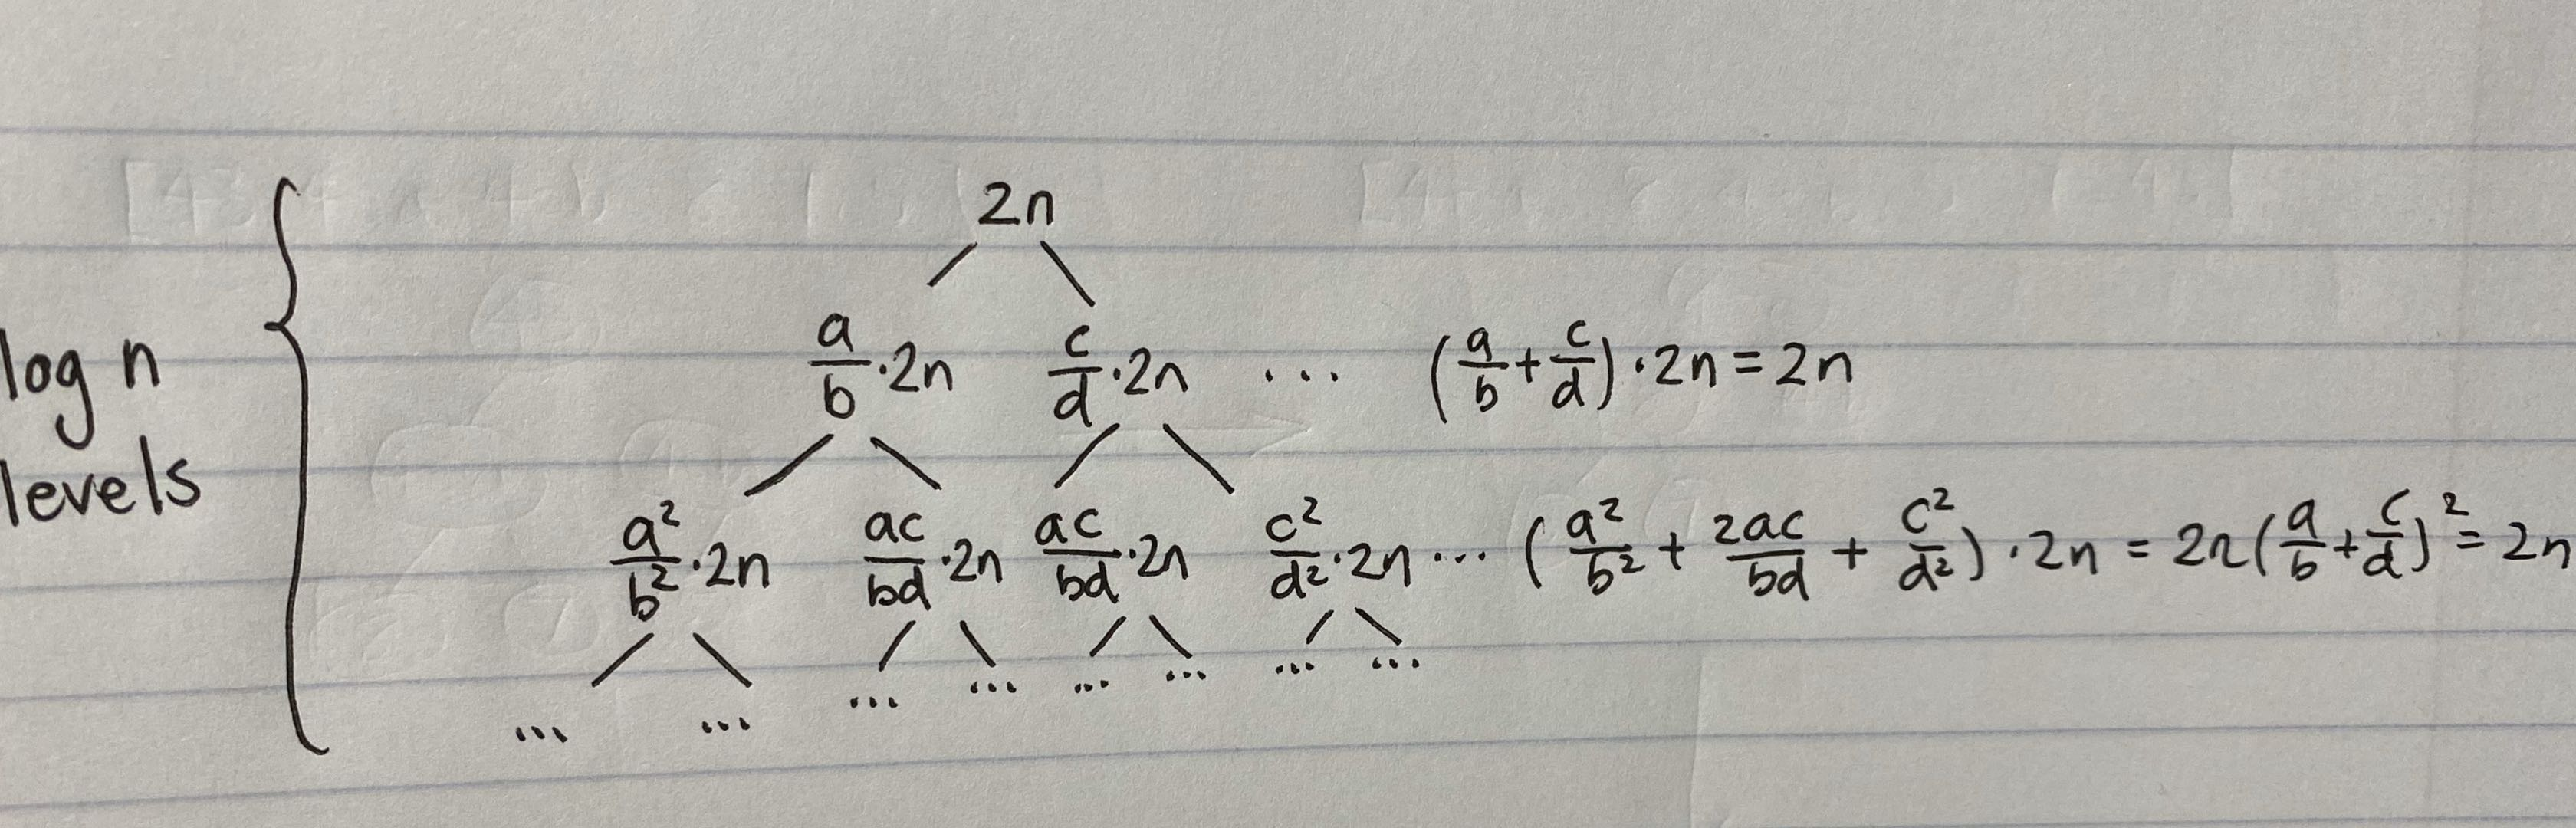
\includegraphics[scale=0.1]{pic1.jpeg}
\vspace*{.25in} % here's how you add some vertical spacing!  Take this out if you don't want it.
% ------ new problem ---------------------------------------------------------------------------------
\begin{problem} Sorting in Linear Time \end{problem}
\begin{enumerate}
    \item Show how to sort $n$ integers in the range $0$ to $n^3 - 1$ in $O(n)$ time.
    \begin{proof}
    We can achieve this by using Radix Sort. Let $n$ be the base of representation and we need to convert each integer to base $n$. This step takes linear run-time. By such a way, the number of digit in largest value $n^3-1$ is $\log_n (n^3-1)=3$. Then we plug $d=3$ and $b=n$ into $O(d(n+b))=O(3*2n)=O(n)$. Overall, the total run-time is $O(n)$.
    \end{proof}
    \item Give a linear-time algorithm to sort the ratios of $n$ given pairs of integers between $1$ and $n$. I.e., we need to sort, within $O(n)$ time, $n$ pairs of the form $(a_i,b_i)$ where $1 \leq  a_i \leq n$ and $1 \leq b_i \leq n$ using the sort key $\frac{a_i}{b_i}$. Prove both run-time and correctness.
    \begin{proof}
    Algorithm: First we need to multiply each ratio by $n^2$ and keep the integer part by $\lfloor \frac{a_i}{b_i}n^2\rfloor$. Then convert each one to base $n$. The match between the original ratio and n-base integer is maintained so later we can use it to transform back to get the original pair. Following this, we apply Radix Sort on the n-base integers and transform them back to get $n$ pairs of form $(a_i, b_i)$ which are sorted accordingly. 
    
    Correctness: The input ratios range from $\frac{1}{n}$ to $n$. After multiplying each ratio by $n^2$ and keeping the integer part, we create a map from the original ratio to integer. The key here is that we need to make sure the map is one-on-one. We know the smallest difference in the original ratio is $\frac{1}{n}-\frac{1}{n-1}=\frac{1}{n(n-1)}$. By multiplying $n^2$, we have $\frac{n}{n-1}>1$, so taking integer part with the floor function will ensure the match is one-on-one. Then we convert the integer to base $n$ for the ready use of Radix Sort. The following part is based on the Radix Sort which will sort the integers. Thus this algorithm can achieve our goal. 
    
    Run-time: The multiplication and conversion steps take linear run-time. In this case, the largest integer is $n^3$ so $d=4$ and $b=n$. Then we have $O(d(n+b))=O(4*2n)=O(n)$ for Radix Sort. The trasnform-back step then takes linear run-time. Overall, we have $O(n)$ total run-time.
    \end{proof}
    \item You are given an array of integers, where different integers may have different numbers of digits, but the total number of digits over \emph{all} the integers in the array is $n$.  Show how to sort the array in $O(n)$ time.
    \begin{proof}
    First we iterate through the array to split integers into different sub arrays based on the number of digits. The number of integers in the array is proportional to $n$ so this step takes $O(n)$ run-time. Since the integer with more digits must be greater than the integer with less digits, we can perform Radix Sort within each sub array (sub arrays are ordered by the number of digits) and the whole array will be sorted. Within each sub array, let us assume that there are $k$ integers with $d$ digits. We use base $10$ as the base of representation for all sub array. Then the run-time to perform Radix array on all sub arrays is 
    \begin{align}
        O(\sum d(k+10))=O(\sum dk+10d)=O(n)
    \end{align}
    where $\sum dk = n$ according to the definition and $\sum 10d$ is proportional to $n$. Therefore, combining the splitting step with Radix Sort, the run-time is $O(n)$. 
    
    \end{proof}
\end{enumerate}

\vspace*{.25in} % here's how you add some vertical spacing!  Take this out if you don't want it.
% ------ new problem ---------------------------------------------------------------------------------
\begin{problem} [Extra Credit] Heap Sort \end{problem}
Demonstrate by example that Heap Sort is not stable.

To illustrate that Heap Sort is not stable, let us consider the array $[43, 40a, 40b, 8, 7, 5]$. For the purpose of demonstration, I use $40a$ and $40b$ to differentiate two $40$s in the array, and they are equal to each other in sorting. 

Then we perform Heap Sort. The array is already in max Heap form, so we swap $43$ with $5$ in the array and remove the node of $43$ in Heap. After creating max Heap, the array becomes $[40a, 8, 40b, 5, 7, 43]$. Then we swap $40a$ with $7$ in the array and remove the node of $40a$ in Heap. After creating max Heap, the array becomes $[40b, 8, 7, 5, 40a, 43]$.
Then we swap $40b$ with $5$ in the array and remove the node of $40b$ in Heap. After creating max Heap, the array becomes $[8, 5, 7, 40b, 40a, 43]$.
Then we swap $8$ with $7$ in the array and remove the node of $8$ in Heap. After creating max Heap, the array becomes $[7, 5, 8, 40b, 40a, 43]$. Then we swap $7$ with $5$ and remove the node of $7$. There is only one node in Heap so the algorithm ends. The output array is $[5, 7, 8, 40b, 40a, 43]$. As we compare the input array and output array, the position of $40a$ and $40b$ is interchanged so Heap Sort is not stable in the example. A graph is attached for illustration.
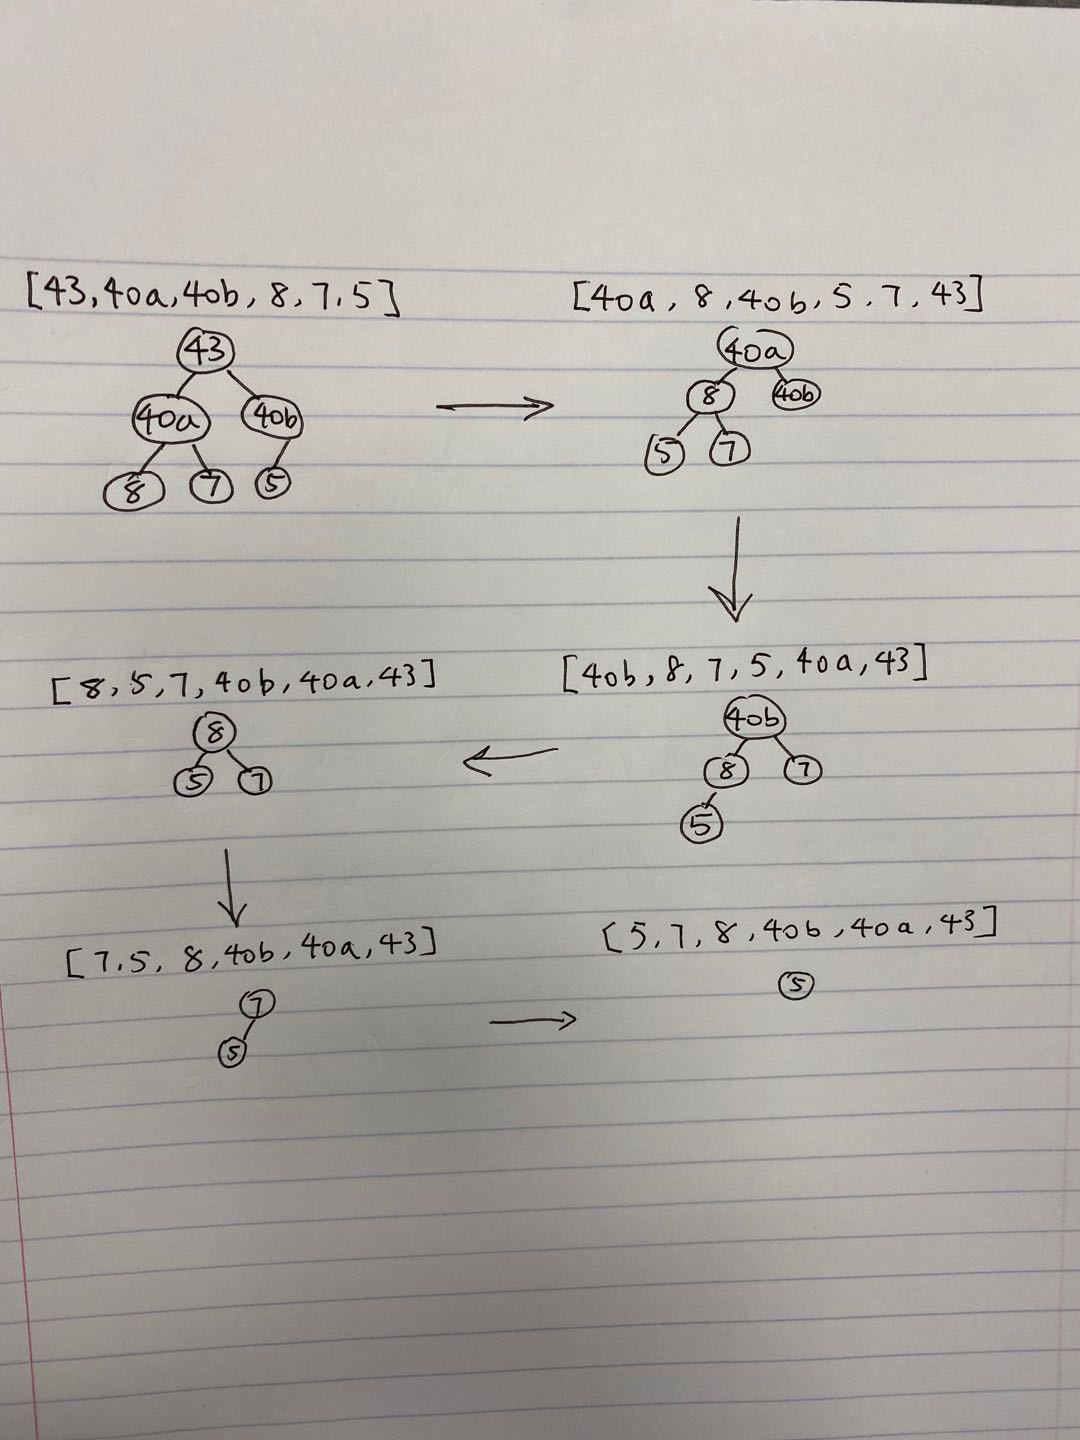
\includegraphics[scale=0.2]{pic2.jpeg}
% Bibliography - uncomment the next two lines to cite your sources!
%\bibliographystyle{plain}
%\bibliography{bibliography}
\end{document}

